\documentclass[12pt]{article}
\usepackage[hmargin={1in},vmargin={1in},foot={.6in}]{geometry} \usepackage{times}
\usepackage{mathrsfs}
\usepackage{textcomp}
\usepackage{xcolor}
\usepackage{amsmath}
\usepackage{tikz}
\usepackage{subcaption}

\usepackage[utf8]{inputenc}
\usepackage{gb4e}

\newcommand{\sem}[1]{\mbox{$[\![$#1$]\!]$}}
\newcommand{\lam}{$\lambda$}
\newcommand{\gcs}[1]{\textcolor{blue}{[gcs: #1]}}
\newcommand{\gnl}[1]{\textcolor{red}{[gnl: #1]}} 
\newcommand{\bej}[1]{\textcolor{magenta}{[bej: #1]}} 

\title{RSA-impf-shift-SuB}
\author{Gunnar Lund}
\date{February 2018}

\begin{document}

%\maketitle


\begin{center}
\textbf{The pragmatics of semantic change: Modeling the progressive-to-imperfective shift}
\end{center}

\vspace{-5pt}
\noindent We implement a computational model of the cyclic progressive-to-imperfective shift, in which languages with a single imperfective marker grammaticize new progressive markers which ultimately broaden in interpretation and displace the older imperfective.  %Our model builds on the presentation of Deo (2015); %who describes the process whereby a language with a single imperfective marker \textsc{impf} is prone to innovate a new progressive marker \textsc{prog}, which ultimately overtakes \textsc{impf} in its range of interpretations.
 %often from an adverbial or periphrastic construction.  Once in this \textit{emergent-\textsc{prog}} stage, \textsc{impf}’s readings narrow, losing the event-in-progress interpretation %one due to scalar implicature, as the language transitions to a \textit{categorical-\textsc{prog}} stage.  Finally, \textsc{prog}’s range of meanings broadens and it ultimately fully displaces \textsc{impf}, completing the cycle.  
While Deo (2015) offers a model of this process within the framework of evolutionary game theory, her model ultimately abandons the semantics she takes such care to construct. Our model offers a more interpretable alternative, operating directly over the semantics.  We show how semantic change may be a function of changes in utterance cost---a reflection of morphological complexity or frequency-of-use---as it relates to pragmatic reasoning. Counter to claims that grammaticization is a process of conventionalization of implicature (Traugott \& Dasher 2002, Traugott \& K\"{o}nig 1991), our model holds the denotations of aspectual markers static; what changes is how we reason about their use given their relative cost. %The pragmatic inference need not be conventionalized at all.
%(Deo (2015) suggests that this final change might occur if a child has an innate bias toward simpler grammars; upon increasingly hearing the utterance PROG, she might mis-generalize it as an imperfective marker [ehh, not a big fan of this phrasing].)  Tigre data taken from Raz (1983) show a contrast between an imperfective marker and a more morphologically complex progressive one; Tigre is between the third and final stages in the cycle just discussed.   While both the imperfective and progressive can have characterizing readings, the imperfective cannot describe events in progress:\\ Tigre data

We adopt a version of Deo's (2009, 2015) semantics, wherein both the imperfective and progressive markers feature universal quantification over a partitioned time interval. \textsc{impf} and \textsc{prog} differ in that the partitioned interval over which \textsc{impf} quantifies is a superinterval of the reference interval, a contextually-determined interval of time relevant to the evaluation of the utterance; \textsc{prog} quantifies over subintervals of the reference interval itself. This difference is illustrated in (\ref{semantics}), where $\mathscr{R}_j^c$ is a regular contextual partition over $j$ and {\sc coin}$(P,k,w)$ holds when $P$ is true at $k$ in $w$. The smaller the partitioned interval, the smaller the partitions are, and the closer each individual partition is to \textit{now}. As a result, events need to be closer to \textit{now} to overlap with each partition cell. The larger the partitioned interval, the further each partition cell is from \textit{now} and the further apart each cell-overlapping event may be. Smaller intervals correspond to event-in-progress readings, as the events are close to \textit{now}; larger intervals correspond to characterizing readings, as events may be far in the future and more sporadically distributed over time. See Fig.~\ref{figure} (\emph{bottom}) for a visual representation of these intervals and interpretations. %our model's representation of this where, e.g, boxes represent partitioned intervals and dots represent events. \gnl{maybe we can save the number line description for later?}

%\gcs{the following explanation still isn't intuitive enough} Event-in-progress readings that characterize progressive aspect arise when the partitioned reference interval is relatively small. The partitions will be small as a result and require the predicate to either hold over the entire interval or several times in quick succession. Characterizing readings typical of imperfective aspect arise when the partitioned interval is large, leading to larger partitions. With larger partitions, the predicate may hold more sporadically over time. Because \textsc{impf} involves a superinterval of the reference interval, it more easily satisfies characterizing scenarios than \textsc{prog}.

\vspace{-8pt}
\begin{exe}
\ex\label{semantics}\begin{xlist}
\ex \sem{\sc impf} = $\lambda P\lambda i\lambda w.\exists j[i \subseteq_{ini} j \wedge \forall k[k \in \mathscr{R}_j^c \to$ {\sc coin}$(P,k,w)]]$
\ex \sem{\sc prog} = $\lambda P\lambda i\lambda w.\forall k[k \in \mathscr{R}_i^c \to$ {\sc coin}$(P,k,w)]]$
\end{xlist}
\end{exe}
\vspace{-8pt}
In a system where both \textsc{prog} and \textsc{impf} are active, given that \textsc{prog} describes a narrower set of scenarios than \textsc{impf}, the use of \textsc{prog} entails \textsc{impf}. This asymmetry leads to a run-of-the-mill scalar implicature whereby the use of \textsc{impf} implies that \textsc{prog} does not hold (a speaker would use the stronger \textsc{prog} if it were true), which suggests that $P$ fails to hold for the contextually-salient reference interval. In other words, the use of \textsc{impf} rules out the narrower set of interpretations \textsc{prog} wold have delivered, which reduces event-in-progress reading for \textsc{impf}. Conversely, the use of %the morphologically more complex 
\textsc{prog} suggests that $P$ does not hold \textit{beyond} the reference interval, ruling out characterizing and habitual readings which extend into the future beyond the reference interval.

We model the pragmatic reasoning that strengthens and refines the interpretations of \textsc{prog} and \textsc{impf} within the Bayesian Rational Speech Act (RSA) framework, where speakers and listeners reason recursively about utterances and the world state those utterances decribe (Frank \& Goodman 2012; Goodman \& Frank 2016). In our model, a ``lifted-variable'' RSA variant, listeners also reason about the reference interval ($I_{ref}$) and superinterval ($I_{sup}$) under discussion. Put differently, our model assumes that listeners have uncertainty about the precise reference and superintervals that are relevant when interpreting utterances that appeal to grammatical aspect. Utterance interpretation involves three levels of inference. At the base, the literal listener ($L_0$) interprets utterances according to their literal semantics; $L_0$ updates beliefs about the state of the world $s$ conditioned on the semantics of $u$ and some specified $I_{ref}$ and $I_{sup}$. One level up, the pragmatic speaker ($S_1$) chooses an utterance $u$ to communicate some observed $s$ to $L_0$. $S_1$ makes this choice by maximizing the probability that $u$ would convey $s$ to $L_0$ while minimizing the utterance cost ($C(u)$); the temperature parameter $\alpha$ controls $S_1$'s optimality when maximizing utterance utility. At the top level of inference, the pragmatic listener ($L_1$) observes $u$ and updates beliefs about $s$, together with the likely values for $I_{ref}$ and $I_{sup}$. Thus, $L_1$ uses $u$ to jointly infer the state of the world and the relevant intervals. $L_1$ performs this inference by reasoning about the probability that  $S_1$ would have chosen $u$ to communicate about $s$ relative to some specific $I_{ref}$ and $I_{sup}$.

\vspace{-7pt}
\begin{exe}
\ex $P_{L_1}(s, I_{ref}, I_{sup} | u) \quad \propto \quad P_{S_1}(u | s, I_{ref}, I_{sup}) \cdot P(s) \cdot P(I_{ref}) \cdot P(I_{sup})$\\
$P_{S_1}(u | s, I_{ref}, I_{sup}) \quad \propto \quad exp(\alpha \cdot [log(P_{L_0}(s | u, I_{ref}, I_{sup})) - C(u)])$\\
$P_{L_0}(s | u, I_{ref}, I_{sup}) \quad \propto \quad \sem{$u$}^{I_{ref}, I_{sup}} \cdot P(s)$
\end{exe}
\vspace{-7pt}
%With this model, we show that the different stages of the progressive-to-imperfective shift correspond to differences in relative utterance costs. 
To generate model predictions, we fix the free parameters of the model. We model states of the world $s$ as sets of numeric values from 0 to 10, corresponding to time indices when the predicate holds (Fig.~\ref{figure}, \emph{bottom}). The possible utterances are \texttt{prog} and \texttt{impf}, which return true when $P$ is true of each partition of the relevant interval $I$; our model also features a \texttt{null} utterance (i.e., saying nothing at all). By manipulating the relative costs of \texttt{prog} and \texttt{impf}, we model their prevalence in a language at a particular stage of aspectual marking. 

The emergent \textsc{prog} stage, where \textsc{prog} constructions are often periphrastic and less frequent, involves \textsc{prog} constructions with a high utterance cost (i.e., morphologically complex and infrequent) relative to that of \textsc{impf} (Bybee et al.~1994, Dahl 1985). %We model this morphological asymmetry with a cost asymmetry for \texttt{prog} vs.~\texttt{impf} (\gcs{specific cost values, or point to table with values}). 
At this stage, \textsc{prog} is used almost exclusively with event-in-progress readings, but its high cost leads to an overall preference for \textsc{impf} for both event-in-progress and characterizing scenarios. As \textsc{prog}'s morphology streamlines, its cost lowers and it gets used more frequently. This leads to the categorical \textsc{prog} stage, where there is a preference for \textsc{prog} to describe event-in-progress readings while \textsc{impf} describes characterizing ones. Here we already see a broadening of \textsc{prog}'s meaning, but the cost symmetry between \textsc{prog} and \textsc{impf} allows each utterance to carve out its own space of usage. 
In the expanding \textsc{prog} stage, \textsc{prog}'s meaning broadens yet more, and the relative cost of \textsc{impf} leads to an overall preference for \textsc{prog} for both event-in-progress and characterizing scenarios; \textsc{prog} has displaced \textsc{impf} in its usage.
\begin{figure}[t!]
\centering
\begin{subfigure}{4.5in}
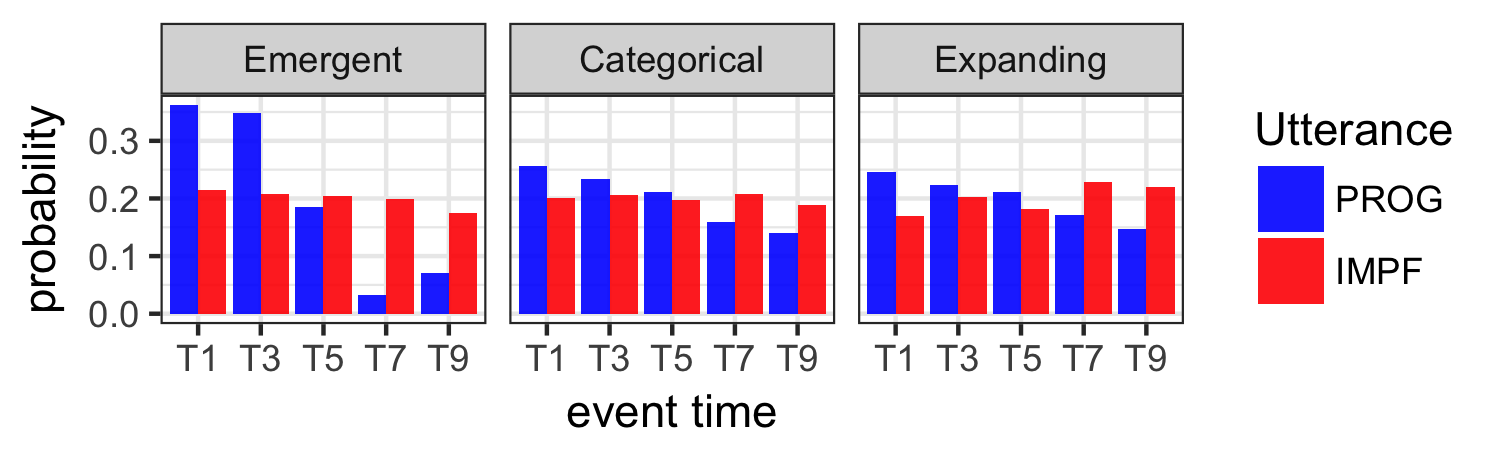
\includegraphics[width=4.5in]{plots/stateprobs.png}
\end{subfigure}
\begin{subfigure}{.3\textwidth}
\begin{tabular}{|c|c|c|} \hline
stage & \textsc{prog} & \textsc{impf} \\ \hline
emergent & 100 & 1 \\
categorical & 1 & 1 \\
expanding & 1 & 100 \\ \hline
\end{tabular}\\
\end{subfigure}

\vspace{-10pt}
\begin{subfigure}{\textwidth}
\centering
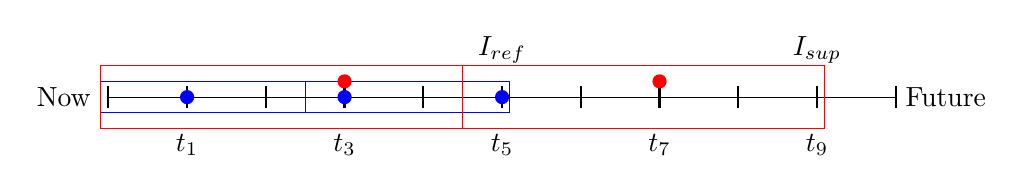
\begin{tikzpicture}
\draw (0,0) -- (10,0);
\draw[blue,thin] (-0.1,-0.2) -- (5.1,-0.2) -- (5.1,0.2) -- (-0.1,0.2) -- (-0.1,-0.2);
\draw[blue,thin] (2.5,0.2) -- (2.5,-0.2);
\draw[red,thin] (-0.1,-0.4) -- (9.1,-0.4) -- (9.1,0.4) -- (-0.1,0.4) -- (-0.1,-0.4);
\draw[red,thin] (4.5,0.4) -- (4.5,-0.4);
\foreach \x in {0,1,2,3,4,5,6,7,8,9,10}
\draw[shift={(\x,0)},color=black,thick] (0pt,4pt) -- (0pt,-4pt);
%\draw (0,-0.35) node[below]{$0$};
\draw (-0.1,0) node[left]{Now};
%\draw (0,-0.35) node[below]{$t_0$};
\draw (1,-0.35) node[below]{$t_1$};
\draw (3,-0.35) node[below]{$t_3$};
\draw (5,0.3) node[above]{$I_{ref}$};
\draw (5,-0.35) node[below]{$t_5$};
\draw (7,-0.35) node[below]{$t_7$};
\draw (9,0.3) node[above]{$I_{sup}$};
\draw (9,-0.35) node[below]{$t_9$};
%\draw (10,-0.35) node[below]{$t_{10}$};
%\draw (10,-0.35) node[below]{$1$};
\draw (10,0) node[right]{Future};

\foreach \i in {1, 3, 5}% points on line
\fill[blue]  (\i,0) circle (0.9 mm);

\foreach \i in {3, 7}% points on line
\fill[red]  (\i,0.2) circle (0.9 mm);
\end{tikzpicture}
\end{subfigure}

\vspace{-11pt}
\caption{\emph{Top left}: model predictions. Probability that the event holds at the specified event time after hearing the \textsc{prog} or \textsc{impf} utterance. \emph{Top right}: relative utterance costs for each stage of aspectual marking. \emph{Bottom}: representation of event-in-progress (blue) and characterizing (red) scenarios, where dots represent events and boxes represent partitioned intervals.}
\label{figure}
\vspace{-15pt}
\end{figure}
Our model thus captures the progressive-to-imperfective shift while reasoning pragmatically about a stable utterance semantics but changing utterance costs. Note that we have used Deo's semantics for theoretical continuity; any semantics with a similar entailment asymmetry between \textsc{prog} and \textsc{impf} would deliver the same qualitative pattern of results.

%\gcs{revise what follows in light of the new plots/tables} By contrast, \textsc{impf} becomes less likely to describe event-in-progress scenarios. In the \textit{emergent}-\textsc{PROG} stage where \textsc{impf} has a relatively low cost, \textsc{impf} is likely to refer to events-in-progress that extend only partially into the future. As the cost of \textsc{prog} lowers, these event-in-progress readings are unlikely, limiting its use to characterizing readings, especially where the predicate holds infrequently or sporadically.

%Relative costs may change due to frequency of use. As the progressive form is used more and more often, it will begin to have a higher prior and thus a lower cost. \textsc{impf} and \textsc{prog} may be used to answer different sets of questions, where \textsc{prog} is suited to discussing the here-and-now (Goldsmith \& Woisetschlaeger 1982). If these are questions that occur far more frequently, the use of \textsc{prog} is correspondingly more frequent. Our model demonstrates that considerations of cost (i.e., prior probability) are crucial for understanding semantic change. \gnl{becky and i will add figs tomorrow}



%\gcs{note about how any semantics would do as long as there's an entailment asymmetry between IMPF and PROG}

%\gnl{this is fairly easy to edit. i'm also wondering if there should be more labels (e.g. labeling events $e1, e2$, etc.)}


\end{document}
